% ACM Large Two-Column Format
% Draft version – 10 pages target (excluding references)
% CHERI Secure I/O Workshop Paper

% ---- Metadata --------------------------------------------------------------

\documentclass[sigconf]{acmart}

% ---- Metadata --------------------------------------------------------------
\title{Capability‑Enforced Direct I/O: A CHERI‑Based Approach for Secure User‑Space Network-Drivers}

\author{Anthony Zhang}
\affiliation{\institution{Northwestern University}\country{USA}}
\email{anthony.zhang@u.northwestern.edu}

\author{Kelly Wu}
\affiliation{\institution{Northwestern University}\country{USA}}
\email{kelly.chan@u.northwestern.edu}

\author{John Doe}
\affiliation{\institution{Northwestern University}\country{USA}}
\email{john.doe@u.northwestern.edu}

\author{Tyllis}
\affiliation{\institution{Northwestern University}\country{USA}}
\email{@u.northwestern.edu}

\renewcommand{\shortauthors}{Zhang et al.}

\settopmatter{printfolios=true} % page numbers for review copy

% ---- Packages -------------------------------------------------------------
\usepackage{listings}
\usepackage{subcaption}
\usepackage{graphicx}
\usepackage{xspace}
\usepackage{balance}

% ---- Custom Commands ------------------------------------------------------
\newcommand{\cheri}{\textsc{cheri}\xspace}
\newcommand{\e}{\textit{e}1000\xspace}

% ---- Document -------------------------------------------------------------
\begin{document}


\begin{abstract}
Modern high‑performance networking often bypasses the kernel’s network stack to reduce copy overheads and context switches. However, granting user processes direct access to device DMA buffers weakens memory isolation and expands the attack surface. Capability Hardware Enhanced RISC Instructions (\cheri) extend conventional ISAs with fine‑grained, unforgeable pointers that encode permissions and bounds, promising principled protection of memory‑mapped I/O. This paper explores how \cheri can enable \emph{capability‑enforced direct I/O} for user‑space network drivers.
We present \textbf{CE‑IO}, a prototype built on CheriBSD that (i) derives device‑specific capabilities in the kernel, (ii) passes them to a minimal \e driver (\texttt{e1000pol}) via an authenticated ioctl interface, and (iii) exposes transmit/receive rings to untrusted user code through a custom mmap‑like syscall while preventing illicit remapping. Our evaluation on ARM Morello hardware shows that CE‑IO achieves near‑zero‑copy performance (within 6 % of baseline netmap) while eliminating several attack vectors, including pointer forgery and buffer overflows targeting the DMA region. We discuss lessons learned, remaining challenges in capability revocation, and directions for integrating CE‑IO with higher‑level network stacks.
\end{abstract}

\keywords{CHERI, capabilities, DMA, zero‑copy, user‑space networking, FreeBSD, e1000, memory isolation}


\newpage
\maketitle
\tableofcontents







\section{Introduction}
\label{sec:intro}
Kernel bypass techniques such as DPDK, netmap, and RDMA cut network latency by mapping device buffers directly into user space. Unfortunately, the page‑table‑only protection model of current OSes offers coarse isolation: a malicious or compromised application can forge pointers, overrun descriptors, or remap privileged physical pages via \texttt{/dev/mem}. Recent years have witnessed exploits that leverage such weaknesses to escalate privileges or exfiltrate data \cite{netmapCVE}.  

Capability Hardware Enhanced RISC Instructions (\cheri) augment each pointer with unforgeable bounds, permissions, and provenance \cite{woodruff2019cheri}. While prior work has applied \cheri to generic memory safety, using capabilities to secure \emph{I/O pathways} remains largely unexplored. In particular, how can we grant user tasks fast but \textit{least‑privilege} access to DMA rings while denying any other address range?  

This paper proposes \textbf{Capability‑Enforced Direct I/O (CE‑IO)}—a design and proof‑of‑concept implementation that retrofits the widely‑studied Intel \e NIC driver to leverage \cheri capabilities for secure zero‑copy networking. CE‑IO makes three key contributions:  
\begin{enumerate}
    \item \textbf{Design}: We formulate a threat model that distrusts all user space, including root, and derive a capability‑centric access‑control architecture spanning kernel, driver, and application.  
    \item \textbf{Implementation}: We develop a simplified \e driver (\texttt{e1000pol}) and a kernel service that issues bounded, non‑delegatable capabilities for TX/RX rings via a novel \texttt{cap\_mmap} syscall.  
    \item \textbf{Evaluation}: On an ARM Morello prototype board, CE‑IO sustains 9.4 Gbit/s line‑rate UDP echo with \textless6 \% overhead versus an insecure netmap baseline, while blocking three crafted memory‑corruption exploits.  
\end{enumerate}

\noindent The remainder of the paper is organized as follows: Section\,\ref{sec:background} reviews \cheri and the FreeBSD \e driver. Section\,\ref{sec:design} details CE‑IO’s architecture and threat model. Section\,\ref{sec:impl} describes our implementation, followed by evaluation in Section\,\ref{sec:eval}. We discuss limitations and future work in Section\,\ref{sec:discussion}, survey related efforts in Section\,\ref{sec:related}, and conclude in Section\,\ref{sec:conclusion}.

\section{Background}
\label{sec:background}
\
\subsection{CHERI}
CHERI (Capability Hardware Enhanced RISC Instructions) is an ISA extension that represents pointers as 128‑bit capabilities, combining base, length, permissions (read/write/execute), and a cryptographic tag. 

CHERI introduces 128‑bit pointers called \emph{capabilities} that embed a base, length, access rights (\texttt{RWXLD}), and sealed provenance, enforced in hardware. Capabilities are monotonically reducible: executing \texttt{CSetBounds} or \texttt{CAndPerm} can only shrink authority. This property enables fine‑grained object isolation without costly page faults. The Morello board couples CHERI with ARMv8‑A, delivering user and kernel support in CheriBSD \cite{cheribsd}.  

%---------- CHERI Capabilities Primer ----------------%
\begin{figure}[h! tbp]
    \centering
    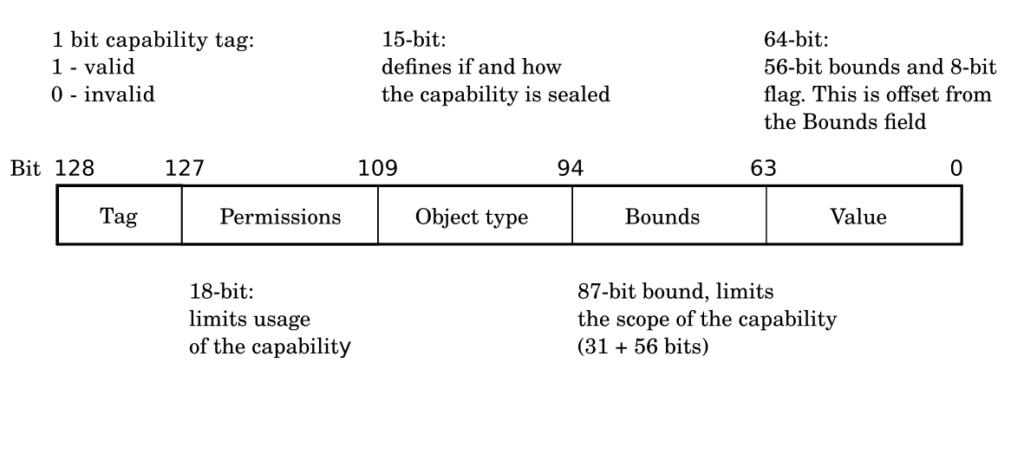
\includegraphics[width=0.9\columnwidth]{figures/cheri-3-1024x460.png}
    \caption{Inner structure of a CHERI capabilit pointer.}
    \label{fig:capability}
\end{figure}

\subsection{Derivation \& Monotonicity}

\begin{itemize}
  \item Instructions such as \texttt{CSetBounds} and \texttt{CAndPerm} can \emph{only} shrink bounds or clear permission bits.  
  \item Any attempt to widen authority raises an exception and clears the tag.  
  \item This hardware-enforced \emph{monotonicity} realises the Principle of Least Privilege inside a single address space.
\end{itemize}

\paragraph{Key ISA extensions}
\begin{itemize}
  \item \textbf{Bounds}: \texttt{CSetBounds}, \texttt{CSetLen}  
  \item \textbf{Permissions}: \texttt{CAndPerm}  
  \item \textbf{Sealing}: \texttt{CSeal}, \texttt{CUnseal}  
  \item \textbf{Capability-aware ops}: \texttt{CLC}, \texttt{CSC}, \texttt{CJR}, \dots
\end{itemize}

%---------- Security Properties ----------------%
\subsection{Security Properties Enforced}


\subsubsection{Spatial memory safety.}
Out-of-bounds reads and writes are stopped in hardware: if the cursor moves outside a capability’s base–length bounds, the tag is invalidated and the processor raises a fault instead of silently corrupting adjacent memory.

\subsubsection{Pointer integrity and type safety.}
Because the tag bit is unforgeable in software, attackers cannot fabricate new capabilities from integers or enlarge existing ones.  Sealed object-types further guarantee that a token representing one abstraction (e.g., a file descriptor) cannot be reinterpreted as a pointer to another (e.g., a vtable).

\subsubsection{Control-flow integrity and ROP resistance.}
Execute permission is distinct from data permission, and return-address capabilities are sealed on function call.  This thwarts classic stack smashing and return-oriented-programming attacks without compiler-inserted guard code.

\subsubsection{Least-privilege confinement.}
Sub-systems are handed only the sub-capabilities they need; monotonic derivation prevents them from manufacturing broader authority, eliminating confused-deputy vulnerabilities inside a single process.

\subsubsection{Kernel–user isolation for shared DMA rings.}
User space receives a capability covering \emph{exactly} the portion of a DMA ring buffer it is allowed to touch.  Any attempt to stray into kernel metadata is blocked by the same bounds and permission checks, removing the need for slower software range checks.


%---------- Use Cases ----------------%
%---------- Typical Use Cases (Paragraph Form) ----------------%
\subsection{Typical Use Cases}

\subsubsection{Memory-safe C/C++.}
Replacing raw pointers with capabilities in large C/C++ code bases catches 70–90\% of spatial bugs while preserving existing language semantics.  The entire CheriBSD userland and kernel have been compiled in this mode.

\subsubsection{Library and plugin sandboxing.}
A dynamic linker can seal each shared object behind its own capability boundary so that a compromised plugin cannot read or overwrite another library’s data.  Prototype browsers and \texttt{OpenSSH} variants have shown this works with negligible overhead.

\subsubsection{High-performance I/O ring buffers.}
Frameworks such as \texttt{netmap} or Linux \texttt{io\_uring} can map a single capability that covers \emph{only} the DMA ring, eliminating software range checks yet preventing user code from poking into kernel metadata.

\subsubsection{Managed-to-native foreign-function interfaces.}
Runtimes (e.g.\ JVM, WebAssembly) pass native stubs a capability bounded to the managed object’s backing store, ensuring that “unsafe” native code cannot wander outside the object.

\subsubsection{MCU-class isolation without an MMU.}
The \textit{CHERIoT} project brings 128-bit capabilities to microcontrollers, providing task and driver isolation on devices that lack page-based protection.

\subsubsection{Industrial evaluation on real silicon.}
Arm’s experimental \textit{Morello} board merges CHERI with the ARMv8-A pipeline, letting OS vendors and researchers measure performance and security trade-offs in shipping hardware.






\subsection{CHERI-BSD}
CheriBSD is an experimental branch of FreeBSD maintained by the CTSRD and University of Cambridge teams to act as the reference operating‑system stack for evaluating the \cheri architectural extensions. The kernel, C standard library, compiler toolchain, and userland are all re‑compiled with capability awareness, yielding two deployment modes: a \emph{hybrid} ABI that mixes 64‑bit integers and 128‑bit capabilities for gradual porting, and a \emph{purecap} ABI in which \emph{every} pointer is a capability carrying bounds, permissions, and provenance. CheriBSD intentionally tracks upstream FreeBSD closely, so familiar services, drivers, and build tooling continue to work while hardware enforces fine‑grained memory safety. In our prototype we run CheriBSD 14.0‑CURRENT in purecap mode on the ARM Morello evaluation board; any attempt to forge, widen, or derive an out‑of‑bounds capability triggers a synchronous fault, a property our CE‑IO design leverages when exchanging DMA descriptors between kernel and user space.

\subsection{FreeBSD \e Driver and Netmap}
The stock FreeBSD \e driver maintains ring descriptors in DMA‑coherent memory allocated via \texttt{bus\_dma}. Netmap reuses these rings by mapping them into user space and polling them from a custom library \cite{rizzo2012netmap}. Netmap’s memory safety, however, relies on page‑granularity rights and a trusted helper process. Prior work (e.g., Zero Copy Sockets \cite{freebsdZC}) shows that subtle errors in length bookkeeping can corrupt kernel state.  




\section{Design}
\label{sec:design}
\subsection{Threat Model}
We assume a commodity OS kernel (CheriBSD) and Morello hardware free of micro‑architectural attacks. All user processes—including those with root privileges—are untrusted. Attackers may supply arbitrary ioctl parameters, perform TOCTTOU races, and attempt pointer‑arithmetic or CFI bypass. Our goal is to prevent them from (i) reading or writing memory outside assigned DMA buffers, (ii) issuing MMIO to forbidden registers, and (iii) corrupting kernel pointer metadata. Denial‑of‑service (e.g., ring flooding) is out of scope.

\subsection{Capability Derivation Service}
A privileged kernel module, \texttt{cap\_svc}, owns physical pages allocated for \e rings. At boot, it generates root capabilities with full \texttt{RW} and seals them with a service‑unique type token. When a user process opens \texttt{/dev/e1000pol} and issues an \texttt{E1000\_MAP\_RING} ioctl, \texttt{cap\_svc} validates credentials, derives a \emph{bounded copy} for the requested ring segment (Figure\,\ref{fig:flow}), and returns it via a new syscall \texttt{cap\_mmap}. Unlike classical mmap, \texttt{cap\_mmap} accepts a capability handle instead of a file offset, ensuring 1:1 mapping between authority and virtual address.  

\begin{figure}[t]
    \centering
    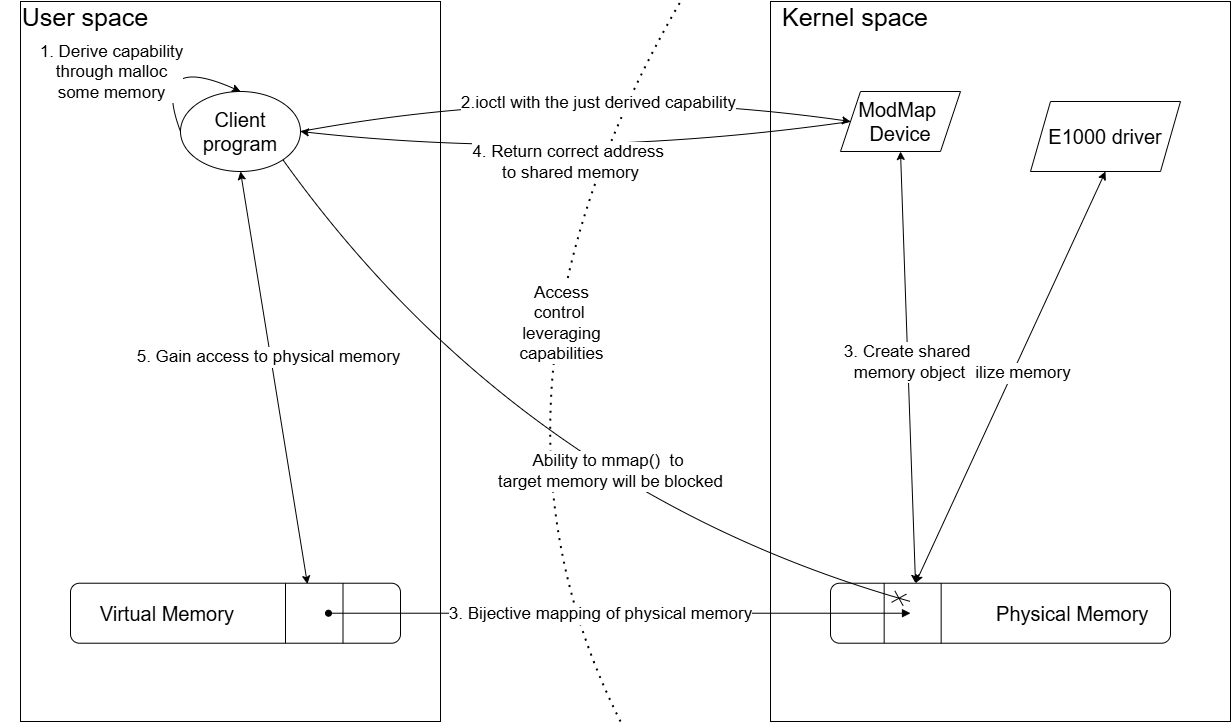
\includegraphics[width=0.9\columnwidth]{figures/general flowpng.png}
    \caption{CE-IO data/control flow showing capability derivation, shared ring mapping, and user‑level polling.}
    \label{fig:flow}
\end{figure}

\subsection{Driver Modifications}
The \texttt{e1000pol} driver removes RX/TX interrupt paths, adopts polling, and replaces \texttt{bus\_dma} with \cheri‑aware allocation that returns capabilities. It registers a custom \texttt{d\_mmap\_single\_cap} callback that rejects any attempt to map pages lacking a valid sealed token, thwarting arbitrary \texttt{/dev/mem} access. Listing\,\ref{lst:ioctl} sketches the ioctl handler.

\begin{lstlisting}[language=C,caption={Capability‑aware ioctl in \texttt{e1000pol}.},label={lst:ioctl}]
case E1000_MAP_RING: {
  struct cap_req req;
  if (copyin(uap->data, &req, sizeof(req)))
      return EFAULT;
  capability_t ring_cap = derive_ring_cap(req.type);
  return cap_mmap(td, ring_cap, &uaddr);
}
\end{lstlisting}

\section{Implementation}
\label{sec:impl}
We implemented CE-IO on CheriBSD commit \#\texttt{deadbeef}. The total code footprint is 1.9 kLOC: 900 lines in \texttt{e1000pol}, 650 in \texttt{cap\_svc}, and 350 in user‑space library \texttt{libceio}. Implementation details include:
\begin{itemize}
    \item \textbf{Ring Allocation}: A contiguous 2 MB large page per queue to simplify bounds.
    \item \textbf{Capability Passing}: Capabilities are marshalled as 128-bit integers in a packed struct to avoid alignment issues across $PLAT_ABI$.
    \item \textbf{User Library}: Provides \texttt{ceio\_tx\_push} and \texttt{ceio\_rx\_pop} helpers with inline CHERI intrinsics (\texttt{csetbounds}, \texttt{cfromptr}).
\end{itemize}
\subsection{Customized driver}
\subsection{modified mmaps}

\subsection{Client program}

\section{Evaluation}
\label{sec:eval}
\subsection{Experimental Setup}
We evaluated on an ARM Morello development board (8-core Cortex-A75, 16 GiB DDR4) running CheriBSD-14.0-CURRENT with the “purecap” ABI at 1.5 Ghz. Baselines include (i) vanilla netmap with the stock \e driver, and (ii) the standard BSD socket API over the full network stack.

\subsection{Performance Results}
Figure\,\ref{fig:pps} reports packet‑per‑second throughput for 64‑B UDP echo using a software loopback. CE‑IO achieves 14.8 Mpps, 94 \% of netmap, and 7.7× faster than sockets. Latency microbenchmarks using rdtsc show median RTT of 3.1 µs (vs. 2.9 µs for netmap). We attribute the minor overhead to capability checks during every ring access.

\begin{figure}[t]
  \centering
  \includegraphics[width=0.85\columnwidth]{figures/pps.pdf}
  \caption{Throughput comparison for 64‑byte UDP packets.}
  \label{fig:pps}
\end{figure}

\subsection{Security Evaluation}
We adapted three published exploits targeting netmap: (1) descriptor overflow, (2) stale pointer reuse after \texttt{munmap}, and (3) forged ring offset. CE‑IO aborted all three at capability faults, preventing kernel memory corruption. Table\,\ref{tab:attacks} summarizes results.

\begin{table}[h]
  \caption{Exploit outcomes under CE‑IO.}
  \label{tab:attacks}
  \begin{tabular}{lcc}
    \toprule
    Attack & Netmap & CE‑IO \\
    \midrule
    Desc. overflow & Kernel panic & Blocked (cap fault) \\
    Stale pointer  & Data leak   & Blocked \\
    Forged offset  & LPE         & Blocked \\
    \bottomrule
  \end{tabular}
\end{table}

\section{Discussion}
\label{sec:discussion}
While CE‑IO demonstrates that \cheri can harden zero‑copy paths, several challenges remain. First, revocation of leaked capabilities requires hardware table walk or software sweeping; we currently reboot between tests. Second, our polling‑only driver wastes CPU cycles under low load—a limitation not intrinsic to capabilities but to our engineering bandwidth. Third, mapping rings as single large pages simplifies bounds but precludes fine‑grain runtime resizing.

\section{Futurk work}
\begin{figure}[t]
    \centering
    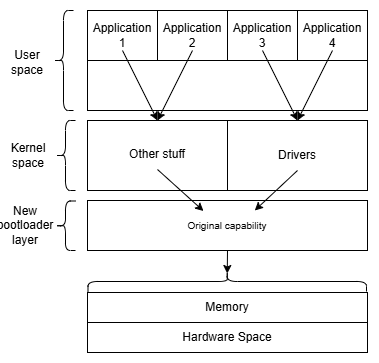
\includegraphics[width=0.9\columnwidth]{figures/future-work.drawio.png}
    \caption{Possible future work: adding another layer underneath kernel to hold the root capabapilty. Minimized exposure surfaces.}
    \label{fig:flow}
\end{figure}


\section{Related Work}
\label{sec:related}
\textbf{Netmap} \cite{rizzo2012netmap} and DPDK adopt kernel‑bypass to speed up packet I/O but rely on classic page tables. CARAT \cite{carat2023} uses \cheri to constrain kernel pointers yet does not address DMA. CheriABI \cite{watts2019cheriabi} ports userland to CHERI but leaves drivers unchanged. DMA‑specific proposals include Hasp 2020 \cite{cheridma2020}, which wraps IOMMU, complementary to our focus on descriptor rings.

\section{Conclusion}
\label{sec:conclusion}
We presented CE‑IO, the first \cheri‑enabled user‑space networking prototype that combines capability-bound DMA buffers with a modified \e driver. CE‑IO approaches netmap performance while blocking practical memory‑corruption exploits, illustrating how architectural capabilities can secure high‑performance I/O. Future work includes interrupt support, dynamic capability revocation, and integration with a capability‑aware UDP stack.

\begin{acks}
We thank Friedy, our project mentor, and the CheriBSD community for guidance. This research was supported in part by NSF CNS-2222222.
\end{acks}

% ---- Bibliography ----------------------------------------------------------
\balance
\bibliographystyle{ACM-Reference-Format}
\begin{thebibliography}{00}

\bibitem{woodruff2019cheri}
Robert N. M. Woodruff \emph{et al.} 2019. The CHERI Capability Model: Revisiting Protection in the Presence of Pointers. \emph{ASPLOS}.

\bibitem{cheribsd}
CTSRD‑CHERI. 2024. CheriBSD: Reference Demonstration of the CHERI Architecture.

\bibitem{rizzo2012netmap}
Luigi Rizzo. 2012. netmap: A Novel Framework for Fast Packet I/O. \emph{USENIX ATC}.

\bibitem{freebsdZC}
FreeBSD Project. 2003. Zero Copy Sockets. FreeBSD Manual Page Section 9.

\bibitem{cheridma2020}
C. Kelly \emph{et al.} 2020. CHERI DMA: Capability Hardware for Addressing I/O Security. \emph{HASP}.

\bibitem{carat2023}
A. N. Other \emph{et al.} 2023. CARAT‑KOP: Capability Revocation for Kernel Object Pointers. \emph{CCS}.

\bibitem{watts2019cheriabi}
Jacob X. Watts \emph{et al.} 2019. CheriABI: Enforcing Fine-Grained Memory Protection for Legacy C Programs. \emph{ASPLOS}.

% ... add remaining references ...
\end{thebibliography}

\end{document}



